%! suppress = MissingLabel
\documentclass[12pt,letterpaper,oneside,reqno]{amsart}
\usepackage{amsfonts}
\usepackage{amsmath}
\usepackage{amssymb}
\usepackage{amsthm}
\usepackage{float}
\usepackage{mathrsfs}
\usepackage{colonequals}
\usepackage[font=small,labelfont=bf]{caption}
\usepackage[left=1in,right=1in,bottom=1in,top=1in]{geometry}
\usepackage[pdfpagelabels,hyperindex,colorlinks=true,linkcolor=blue,urlcolor=magenta,citecolor=green]{hyperref}
\usepackage{graphicx}
\linespread{1.7}
\emergencystretch=1em
\usepackage{array}
\usepackage{etoolbox}
\apptocmd{\sloppy}{\hbadness 10000\relax}{}{}
\raggedbottom

\newcommand \anglePower [2]{\langle #1 \rangle \sp{#2}}
\newcommand \bernoulli [2][B] {{#1}\sb{#2}}
\newcommand \curvePower [2]{\{#1\}\sp{#2}}
\newcommand \coeffA [3][A] {{\mathbf{#1}} \sb{#2,#3}}
\newcommand \polynomialP [4][P]{{#1}(#2,#3,#4)}
\newcommand \polynomialQ [4][Q]{{#1}(#2,#3,#4)}

% ~~~ Rascal numbers ~~~
%\newcommand \rascalNumber [3] {\binom{#1}{#2}_{#3}}
%\newcommand \north[0] {\mathbf{North}}
%\newcommand \south[0] {\mathbf{South}}
%\newcommand \west[0] {\mathbf{West}}
%\newcommand \east[0] {\mathbf{East}}

% ~~~~ 1-q pascal notation~~~~
%\newcommand{\genstirlingI}[3]{%
%    \genfrac{[}{]}{0pt}{#1}{#2}{#3}%
%}
%\newcommand{\genstirlingII}[3]{%
%    \genfrac{\{}{\}}{0pt}{#1}{#2}{#3}%
%}
%\newcommand{\oneQBinomial}[3]{\genstirlingI{}{#1}{#2}^{#3}}

% free foot note
%\let\svthefootnote\thefootnote
%\newcommand\freefootnote[1]{%
%    \let\thefootnote\relax%
%    \footnotetext{#1}%
%    \let\thefootnote\svthefootnote%
%}


\newtheorem{theorem}{Theorem}[section]
\newtheorem{corollary}[theorem]{Corollary}
\newtheorem{lemma}[theorem]{Lemma}
\newtheorem{example}[theorem]{Example}
\newtheorem{conjecture}[theorem]{Conjecture}
\newtheorem{definition}[theorem]{Definition}

%\numberwithin{equation}{section}

\title[Plots of Closed Forms]
{Plots of Closed Forms}
\author[Petro Kolosov]{Petro Kolosov}
%\address{Software Developer, DevOps Engineer}
%\email{kolosovp94@gmail.com}
%\urladdr{https://kolosovpetro.github.io}
%\keywords{
%    Binomial theorem,
%    Binomial coefficients,
%    Faulhaber's formula,
%    Polynomials,
%    Pascal's triangle
%    Finite differences,
%    Interpolation,
%    Polynomial identities
%}
%\subjclass[2010]{26E70, 05A30}
\date{\today}
\hypersetup{
    pdftitle={LaTeX Template for Github},
    pdfsubject={
        Polynomials,
        Finite differences,
        Interpolation,
        Approximation,
        Polynomial identities,
        Power sums,
        Binomial theorem,
        Power function,
        Binomial coefficients,
        Bernoulli numbers,
        Pascal's triangle,
        Faulhaber's formula,
        Derivatives,
        Differential calculus,
        Partial differential equations,
        OEIS,
        Bernoulli polynomials,
        Combinatorics,
        Discrete convolution,
        Dynamic systems,
        Time scales
    },
    pdfauthor={Petro Kolosov},
    pdfkeywords={
        Polynomials,
        Finite differences,
        Interpolation,
        Approximation,
        Polynomial identities,
        Power sums,
        Binomial theorem,
        Power function,
        Binomial coefficients,
        Bernoulli numbers,
        Pascal's triangle,
        Faulhaber's formula,
        Derivatives,
        Differential calculus,
        Partial differential equations,
        OEIS,
        Bernoulli polynomials,
        Combinatorics,
        Discrete convolution,
        Dynamic systems,
        Time scales
    }
}
\begin{document}
%    \begin{abstract}
%        Your abstract here.
%    \end{abstract}

    \maketitle

    \tableofcontents

%    \freefootnote{Sources: \url{https://github.com/kolosovpetro/github-latex-template}}

    \section{Introduction}\label{sec:introduction}
    \begin{align*}
        \polynomialP{m}{b}{x} &= \sum_{r=0}^{m} \sum_{k=1}^{n} \coeffA{m}{r} k^r (n-k)^r \\
        \polynomialQ{m}{b}{x} &= \sum_{r=0}^{m} \sum_{k=0}^{n-1} \coeffA{m}{r} k^r (n-k)^r
    \end{align*}

    \subsection{Polynomials P(1,n,k)}
    
\begin{align*}
    \polynomialP{1}{X}{0} &= 0 \\
    \polynomialP{1}{X}{1} &= 6X - 5 \\
    \polynomialP{1}{X}{2} &= 18X - 28 \\
    \polynomialP{1}{X}{3} &= 36X - 81 \\
    \polynomialP{1}{X}{4} &= 60X - 176 \\
    \polynomialP{1}{X}{5} &= 90X - 325 \\
    \polynomialP{1}{X}{6} &= 126X - 540 \\
    \polynomialP{1}{X}{7} &= 168X - 833 \\
    \polynomialP{1}{X}{8} &= 216X - 1216 \\
    \polynomialP{1}{X}{9} &= 270X - 1701 \\
    \polynomialP{1}{X}{10} &= 330X - 2300 \\
    \polynomialP{1}{X}{11} &= 396X - 3025 \\
    \polynomialP{1}{X}{12} &= 468X - 3888 \\
    \polynomialP{1}{X}{13} &= 546X - 4901 \\
    \polynomialP{1}{X}{14} &= 630X - 6076 \\
    \polynomialP{1}{X}{15} &= 720X - 7425 \\
    \polynomialP{1}{X}{16} &= 816X - 8960 \\
    \polynomialP{1}{X}{17} &= 918X - 10693 \\
    \polynomialP{1}{X}{18} &= 1026X - 12636 \\
    \polynomialP{1}{X}{19} &= 1140X - 14801 \\
    \polynomialP{1}{X}{20} &= 1260X - 17200
\end{align*}
\begin{figure}[H]
    \centering
    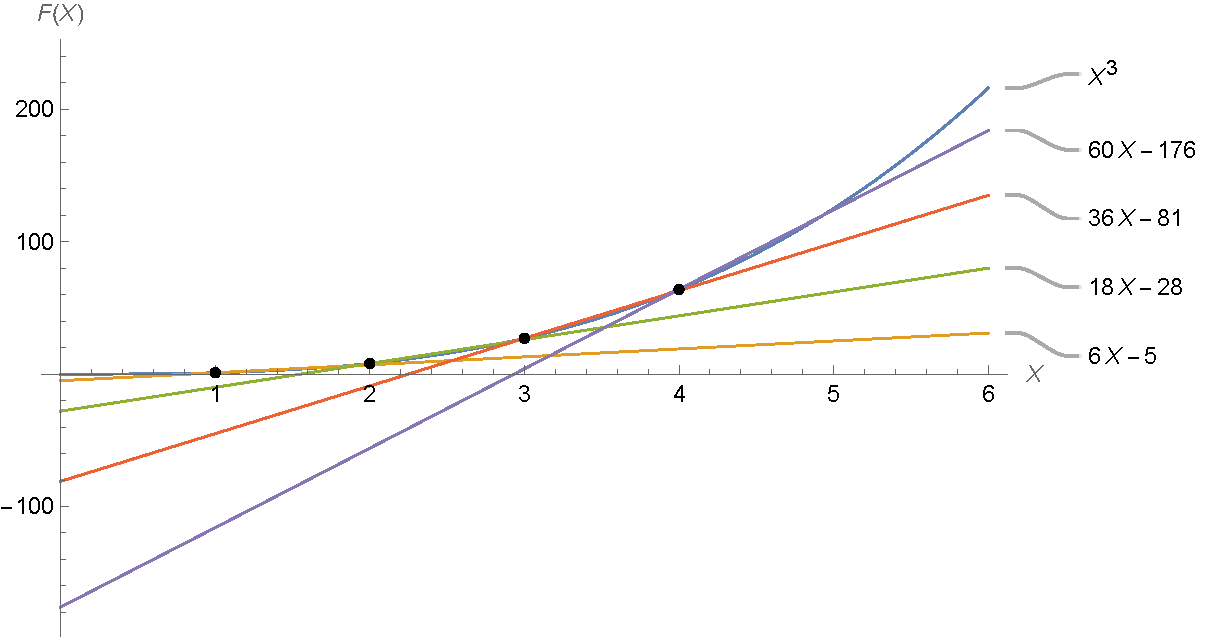
\includegraphics[width=1\textwidth]{sections/images/01_cubes_with_p_1_n_k}
    ~\caption{Polynomials P(1, n, k)}\label{fig:figure}
\end{figure}


    \subsection{Polynomials Q(1,n,k)}
    \begin{align*}
    \polynomialQ{1}{X}{0} &= 0 \\
    \polynomialQ{1}{X}{1} &= 1 \\
    \polynomialQ{1}{X}{2} &= 6X - 4 \\
    \polynomialQ{1}{X}{3} &= 18X - 27 \\
    \polynomialQ{1}{X}{4} &= 36X - 80 \\
    \polynomialQ{1}{X}{5} &= 60X - 175 \\
    \polynomialQ{1}{X}{6} &= 90X - 324 \\
    \polynomialQ{1}{X}{7} &= 126X - 539 \\
    \polynomialQ{1}{X}{8} &= 168X - 832 \\
    \polynomialQ{1}{X}{9} &= 216X - 1215 \\
    \polynomialQ{1}{X}{10} &= 270X - 1700 \\
    \polynomialQ{1}{X}{11} &= 330X - 2299 \\
    \polynomialQ{1}{X}{12} &= 396X - 3024 \\
    \polynomialQ{1}{X}{13} &= 468X - 3887 \\
    \polynomialQ{1}{X}{14} &= 546X - 4900 \\
    \polynomialQ{1}{X}{15} &= 630X - 6075 \\
    \polynomialQ{1}{X}{16} &= 720X - 7424 \\
    \polynomialQ{1}{X}{17} &= 816X - 8959 \\
    \polynomialQ{1}{X}{18} &= 918X - 10692 \\
    \polynomialQ{1}{X}{19} &= 1026X - 12635 \\
    \polynomialQ{1}{X}{20} &= 1140X - 14800
\end{align*}
\begin{figure}[H]
    \centering
    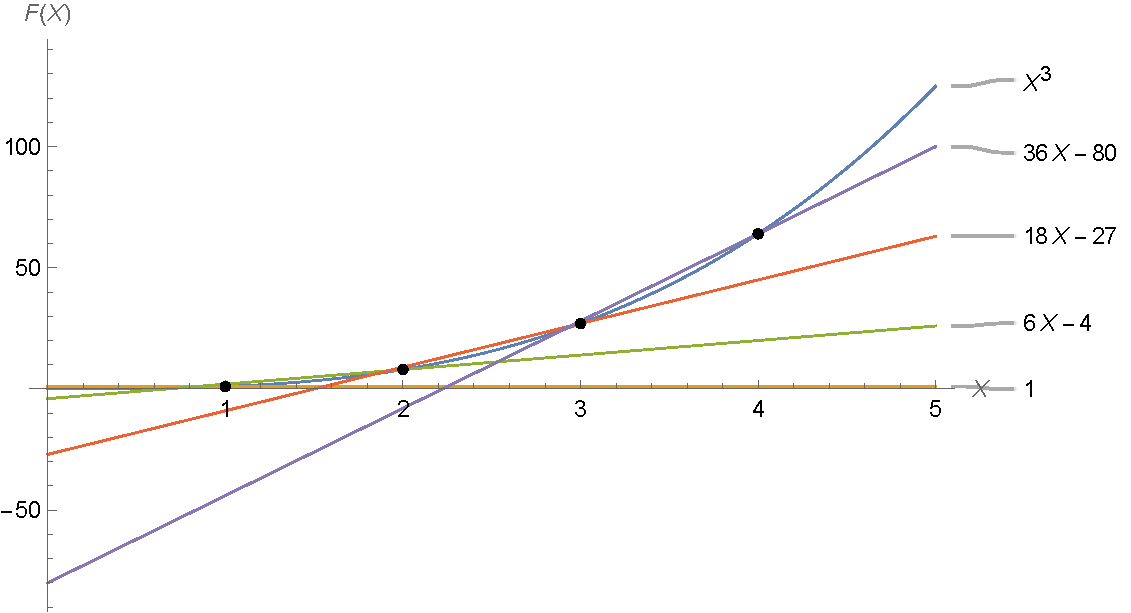
\includegraphics[width=1\textwidth]{sections/images/02_cubes_with_q_1_n_k}
    ~\caption{Polynomials Q(1, n, k)}\label{fig:figure2}
\end{figure}



    \subsection{Polynomials P(2,n,k)}
    \begin{align*}
    \polynomialP{2}{X}{0} &= 0 \\
    \polynomialP{2}{X}{1} &= 30X^2 - 60X + 31 \\
    \polynomialP{2}{X}{2} &= 150X^2 - 540X + 512 \\
    \polynomialP{2}{X}{3} &= 420X^2 - 2160X + 2943 \\
    \polynomialP{2}{X}{4} &= 900X^2 - 6000X + 10624 \\
    \polynomialP{2}{X}{5} &= 1650X^2 - 13500X + 29375 \\
    \polynomialP{2}{X}{6} &= 2730X^2 - 26460X + 68256 \\
    \polynomialP{2}{X}{7} &= 4200X^2 - 47040X + 140287 \\
    \polynomialP{2}{X}{8} &= 6120X^2 - 77760X + 263168 \\
    \polynomialP{2}{X}{9} &= 8550X^2 - 121500X + 459999 \\
    \polynomialP{2}{X}{10} &= 11550X^2 - 181500X + 760000 \\
    \polynomialP{2}{X}{11} &= 15180X^2 - 261360X + 1199231 \\
    \polynomialP{2}{X}{12} &= 19500X^2 - 365040X + 1821312 \\
    \polynomialP{2}{X}{13} &= 24570X^2 - 496860X + 2678143 \\
    \polynomialP{2}{X}{14} &= 30450X^2 - 661500X + 3830624 \\
    \polynomialP{2}{X}{15} &= 37200X^2 - 864000X + 5349375 \\
    \polynomialP{2}{X}{16} &= 44880X^2 - 1109760X + 7315456 \\
    \polynomialP{2}{X}{17} &= 53550X^2 - 1404540X + 9821087 \\
    \polynomialP{2}{X}{18} &= 63270X^2 - 1754460X + 12970368 \\
    \polynomialP{2}{X}{19} &= 74100X^2 - 2166000X + 16879999 \\
    \polynomialP{2}{X}{20} &= 86100X^2 - 2646000X + 21680000
\end{align*}
\begin{figure}[H]
    \centering
    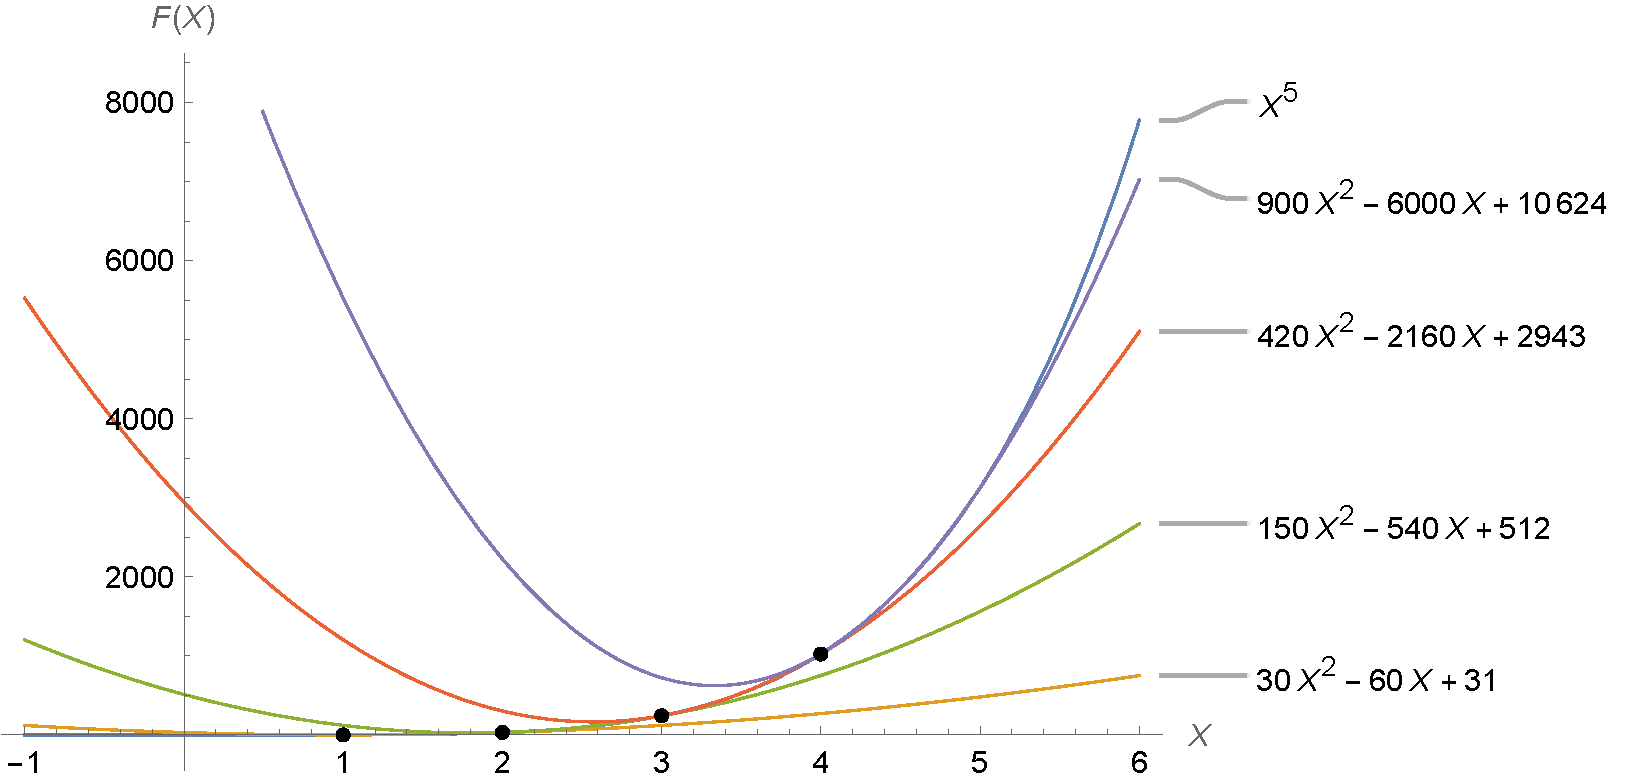
\includegraphics[width=1\textwidth]{sections/images/03_fifth_power_with_p_1_n_k}
    ~\caption{Polynomials P(2, n, k)}\label{fig:figure3}
\end{figure}


    \subsection{Polynomials Q(2,n,k)}
    \begin{align*}
    \polynomialQ{2}{N}{0} &= 0 \\
    \polynomialQ{2}{N}{1} &= 1 \\
    \polynomialQ{2}{N}{2} &= 30N^2 - 60N + 32 \\
    \polynomialQ{2}{N}{3} &= 150N^2 - 540N + 513 \\
    \polynomialQ{2}{N}{4} &= 420N^2 - 2160N + 2944 \\
    \polynomialQ{2}{N}{5} &= 900N^2 - 6000N + 10625 \\
    \polynomialQ{2}{N}{6} &= 1650N^2 - 13500N + 29376 \\
    \polynomialQ{2}{N}{7} &= 2730N^2 - 26460N + 68257 \\
    \polynomialQ{2}{N}{8} &= 4200N^2 - 47040N + 140288 \\
    \polynomialQ{2}{N}{9} &= 6120N^2 - 77760N + 263169 \\
    \polynomialQ{2}{N}{10} &= 8550N^2 - 121500N + 460000 \\
    \polynomialQ{2}{N}{11} &= 11550N^2 - 181500N + 760001 \\
    \polynomialQ{2}{N}{12} &= 15180N^2 - 261360N + 1199232 \\
    \polynomialQ{2}{N}{13} &= 19500N^2 - 365040N + 1821313 \\
    \polynomialQ{2}{N}{14} &= 24570N^2 - 496860N + 2678144 \\
    \polynomialQ{2}{N}{15} &= 30450N^2 - 661500N + 3830625 \\
    \polynomialQ{2}{N}{16} &= 37200N^2 - 864000N + 5349376 \\
    \polynomialQ{2}{N}{17} &= 44880N^2 - 1109760N + 7315457 \\
    \polynomialQ{2}{N}{18} &= 53550N^2 - 1404540N + 9821088 \\
    \polynomialQ{2}{N}{19} &= 63270N^2 - 1754460N + 12970369 \\
    \polynomialQ{2}{N}{20} &= 74100N^2 - 2166000N + 16880000
\end{align*}
\begin{figure}[H]
    \centering
    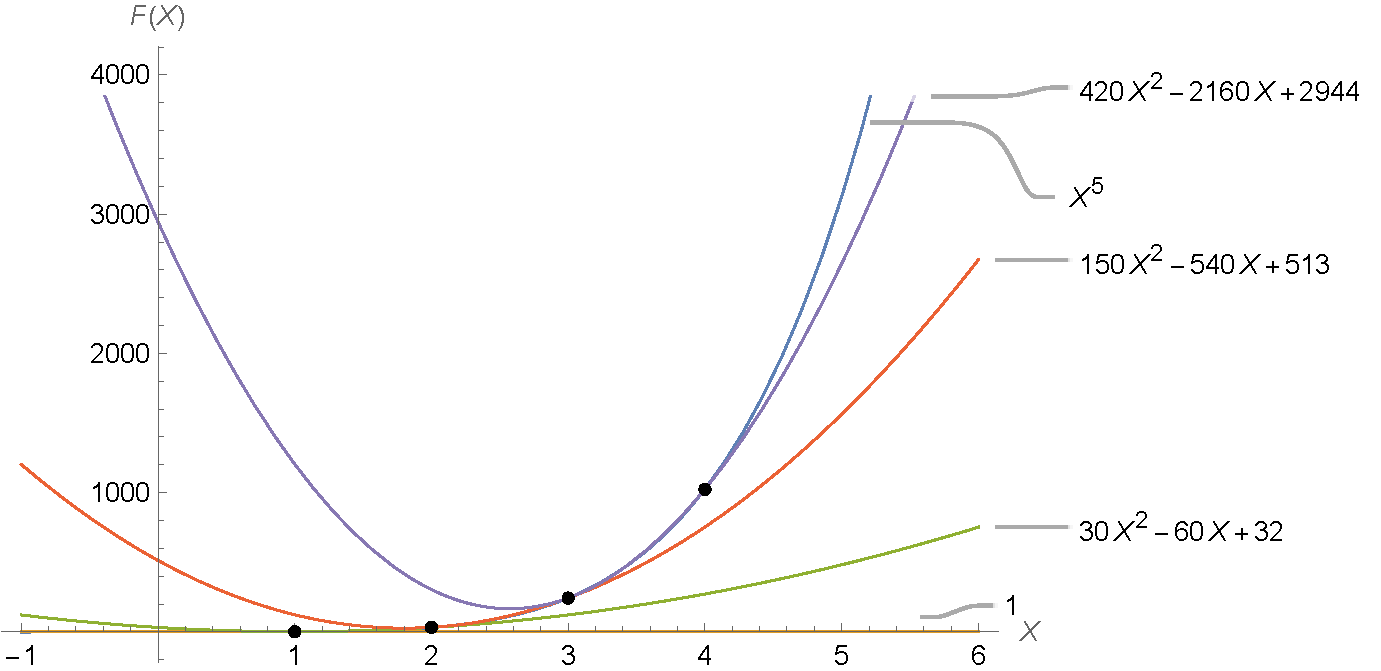
\includegraphics[width=1\textwidth]{sections/images/04_fifth_power_with_q_1_n_k}
    ~\caption{Polynomials P(2, n, k)}\label{fig:figure4}
\end{figure}



    \bibliographystyle{unsrt}
    \bibliography{PlotsOfClosedForms}

\end{document}
